\documentclass{beamer}
\usepackage{tikz}
\usetikzlibrary{arrows.meta, positioning}

\begin{document}

\begin{frame}{Interaction Between Two Parties}

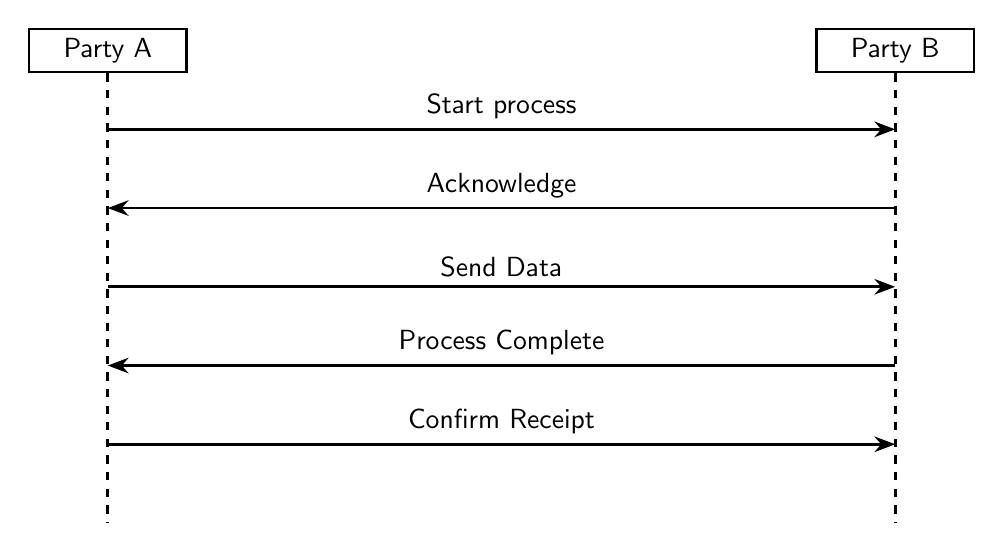
\begin{tikzpicture}[>=Stealth, font=\sffamily, line width=1pt]

  % Party nodes
  \node[rectangle, draw, align=center, minimum width=2cm] (A) at (0,0) {Party A};
  \node[rectangle, draw, align=center, minimum width=2cm] (B) at (10,0) {Party B};

  % Lifelines
  \draw[dashed] (A) -- ++(0,-6);
  \draw[dashed] (B) -- ++(0,-6);

  % Messages
  \draw[->] (A) ++(0,-1) -- ++(10,0) node[midway, above] {Start process};
  \draw[->] (B) ++(0,-2) -- ++(-10,0) node[midway, above] {Acknowledge};
  \draw[->] (A) ++(0,-3) -- ++(10,0) node[midway, above] {Send Data};
  \draw[->] (B) ++(0,-4) -- ++(-10,0) node[midway, above] {Process Complete};
  \draw[->] (A) ++(0,-5) -- ++(10,0) node[midway, above] {Confirm Receipt};

\end{tikzpicture}

\end{frame}

\end{document}
